\PassOptionsToPackage{unicode=true}{hyperref} % options for packages loaded elsewhere
\PassOptionsToPackage{hyphens}{url}
\documentclass[ignorenonframetext,]{beamer}
\setbeamertemplate{caption}[numbered]
\setbeamertemplate{caption label separator}{: }
\setbeamercolor{caption name}{fg=normal text.fg}
\beamertemplatenavigationsymbolsempty
\usepackage{lmodern}
\usepackage{amssymb,amsmath}
\usepackage{ifxetex,ifluatex}
\usepackage{fixltx2e} % provides \textsubscript
\ifnum 0\ifxetex 1\fi\ifluatex 1\fi=0 % if pdftex
  \usepackage[T1]{fontenc}
  \usepackage[utf8]{inputenc}
\else % if luatex or xelatex
  \ifxetex
    \usepackage{mathspec}
  \else
    \usepackage{fontspec}
\fi
\defaultfontfeatures{Ligatures=TeX,Scale=MatchLowercase}







\fi

  \usetheme[]{metropolis}






% use upquote if available, for straight quotes in verbatim environments
\IfFileExists{upquote.sty}{\usepackage{upquote}}{}
% use microtype if available
\IfFileExists{microtype.sty}{%
  \usepackage{microtype}
  \UseMicrotypeSet[protrusion]{basicmath} % disable protrusion for tt fonts
}{}


\newif\ifbibliography


\hypersetup{
      pdftitle={Predicting Hit Songs},
        pdfauthor={Frank K. Saforo; Chris J. Ezelle},
          pdfborder={0 0 0},
    breaklinks=true}
%\urlstyle{same}  % Use monospace font for urls







% Prevent slide breaks in the middle of a paragraph:
\widowpenalties 1 10000
\raggedbottom

  \AtBeginPart{
    \let\insertpartnumber\relax
    \let\partname\relax
    \frame{\partpage}
  }
  \AtBeginSection{
    \ifbibliography
    \else
      \let\insertsectionnumber\relax
      \let\sectionname\relax
      \frame{\sectionpage}
    \fi
  }
  \AtBeginSubsection{
    \let\insertsubsectionnumber\relax
    \let\subsectionname\relax
    \frame{\subsectionpage}
  }



\setlength{\parindent}{0pt}
\setlength{\parskip}{6pt plus 2pt minus 1pt}
\setlength{\emergencystretch}{3em}  % prevent overfull lines
\providecommand{\tightlist}{%
  \setlength{\itemsep}{0pt}\setlength{\parskip}{0pt}}

  \setcounter{secnumdepth}{0}



  \title[]{Predicting Hit Songs}

  \subtitle{Hot 100 Billboard Chart}

  \author[
        Frank K. Saforo \and Chris J. Ezelle
    ]{Frank K. Saforo \and Chris J. Ezelle}


\date[
      \today
  ]{
      \today
        }

\begin{document}

% Hide progress bar and footline on titlepage
  \begin{frame}[plain]
  \titlepage
  \end{frame}



\begin{frame}{Overview}
\protect\hypertarget{overview}{}

\begin{itemize}
\item
  Introduction
\item
  The Data and EDA
\item
  Model Building and Evaluation
\item
  Results and Interpretation
\item
  Recommendation and Conclusion
\end{itemize}

\end{frame}

\begin{frame}{Introduction}
\protect\hypertarget{introduction}{}

\begin{itemize}
\tightlist
\item
  Data was extracted from the Spotify API
\item
  Get out of bed
\end{itemize}

\end{frame}

\hypertarget{the-data}{%
\section{The Data}\label{the-data}}

\begin{frame}{Collecting the Data}
\protect\hypertarget{collecting-the-data}{}

\begin{center}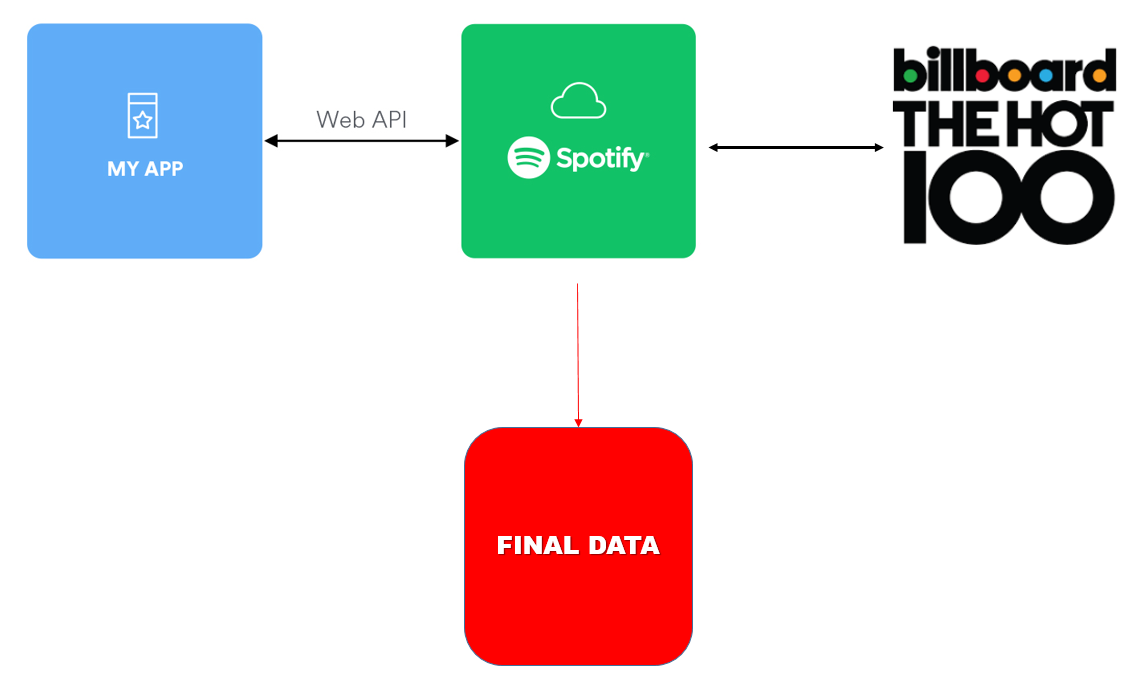
\includegraphics[width=1\linewidth]{./Slides/prz_000} \end{center}

\begin{itemize}
\tightlist
\item
  \textbf{Latest data retrieval was on December 28, 2018}
\end{itemize}

\end{frame}

\begin{frame}[fragile]{Data Snap}
\protect\hypertarget{data-snap}{}

\begin{verbatim}
## 'data.frame':    116372 obs. of  25 variables:
##  $ artist_name     : Factor w/ 32105 levels "'Dwellers","'Lgado",..: 2005 7823 2619 18797 29586 15958 11603 23036 31324 25793 ...
##  $ track_id        : Factor w/ 116191 levels "0009UBVA8DCDwk1Hepib6P",..: 40722 72528 15225 33984 43501 112109 84094 17369 37845 28857 ...
##  $ track_name      : Factor w/ 96809 levels "'03","'84","'89 Chevy",..: 81715 80703 53924 36049 73731 96702 94461 79268 7262 54642 ...
##  $ acousticness    : num  0.28 0.153 0.0141 0.191 0.00513 0.071 0.297 0.551 0.0302 0.194 ...
##  $ danceability    : num  0.724 0.841 0.817 0.687 0.834 0.826 0.752 0.753 0.703 0.729 ...
##  $ duration_ms     : int  207333 212500 210368 214290 312820 225199 201661 158053 198903 183907 ...
##  $ energy          : num  0.647 0.798 0.539 0.792 0.73 0.615 0.488 0.498 0.723 0.625 ...
##  $ instrumentalness: num  0.00 3.33e-06 4.96e-04 0.00 0.00 0.00 9.11e-06 0.00 2.06e-06 9.86e-03 ...
##  $ key             : int  1 1 6 5 8 8 6 2 9 4 ...
##  $ liveness        : num  0.102 0.0618 0.099 0.167 0.124 0.0965 0.0936 0.0706 0.126 0.248 ...
##  $ loudness        : num  -5.64 -4.21 -6.35 -2.75 -3.71 ...
##  $ mode            : int  1 0 0 1 1 0 1 1 0 1 ...
##  $ speechiness     : num  0.0658 0.229 0.0621 0.0452 0.222 0.219 0.0705 0.0504 0.0412 0.0315 ...
##  $ tempo           : num  107 95.9 97.1 100 155 ...
##  $ time_signature  : int  4 4 4 4 4 4 4 4 4 4 ...
##  $ valence         : num  0.435 0.591 0.158 0.671 0.446 0.543 0.533 0.927 0.288 0.261 ...
##  $ popularity      : int  100 99 97 96 95 95 95 95 94 93 ...
##  $ target          : Factor w/ 2 levels "0","1": 2 2 2 2 2 2 2 2 2 2 ...
##  $ tone            : chr  "major" "minor" "minor" "major" ...
##  $ scale           : chr  "C#" "C#" "F" "E#" ...
##  $ keys            : chr  "C# major" "C# minor" "F minor" "E# major" ...
##  $ keysign         : chr  "F,A,C,G,D,A,E,B Sharp" "F,A,G,D Sharp" "B,A,D,E Flat" "B Flat" ...
##  $ keylabel        : chr  "C sharp major: Fullness, Sonorousness, Euphony" "C sharp minor : Despair, Wailing, Weeping" "F minor: Obscure, Plaintive, Funereal" "F major: Complaisance and calm" ...
##  $ tempoc          : chr  "Andante" "Andante" "Andante" "Andante" ...
##  $ tlabel          : chr  "76-108" "76-108" "76-108" "76-108" ...
\end{verbatim}

\begin{verbatim}
## 40.4 MB
\end{verbatim}

\end{frame}

\begin{frame}{The Data\ldots{}}
\protect\hypertarget{the-data-1}{}

\begin{itemize}
\tightlist
\item
  Tempo: Beats Per Minute (BPM) of the song.\\
\item
  Energy: The energy of a song, the higher the value, the more
  energetic.\\
\item
  Danceability: The higher the value, the easier it is to dance to this
  song.\\
\item
  Loudness: The higher the value, the louder the song (in dB).\\
\item
  Valence: The higher the value, the more positive mood for the song.\\
\item
  Length: The duration of the song.\\
\item
  Acousticness: The higher the value the more acoustic the song is.\\
\item
  Release Year: The year each song was released.\\
\item
  \textbf{Popularity (Target Variable)}: The higher the value (on a
  scale of 0 to 100) the more popular the song is.
\end{itemize}

\textbf{Source:} See features description
\href{http://static.echonest.com/SortYourMusic/}{here}

\end{frame}

\hypertarget{exploratory-data-analysis}{%
\section{Exploratory Data Analysis}\label{exploratory-data-analysis}}

\begin{frame}{Most Popular Songs of 2018}
\protect\hypertarget{most-popular-songs-of-2018}{}

\begin{center}\includegraphics[width=1\linewidth]{Li_PrezPDF_files/figure-beamer/unnamed-chunk-4-1} \end{center}

\end{frame}

\begin{frame}{Top 100 Songs by Key}
\protect\hypertarget{top-100-songs-by-key}{}

\begin{center}\includegraphics[width=1\linewidth]{Li_PrezPDF_files/figure-beamer/unnamed-chunk-5-1} \end{center}

\end{frame}

\begin{frame}{Top 100 Songs by Key and Emotion}
\protect\hypertarget{top-100-songs-by-key-and-emotion}{}

\begin{center}\includegraphics[width=1\linewidth]{Li_PrezPDF_files/figure-beamer/unnamed-chunk-6-1} \end{center}

\end{frame}

\begin{frame}{Are danceable songs popular?}
\protect\hypertarget{are-danceable-songs-popular}{}

\begin{center}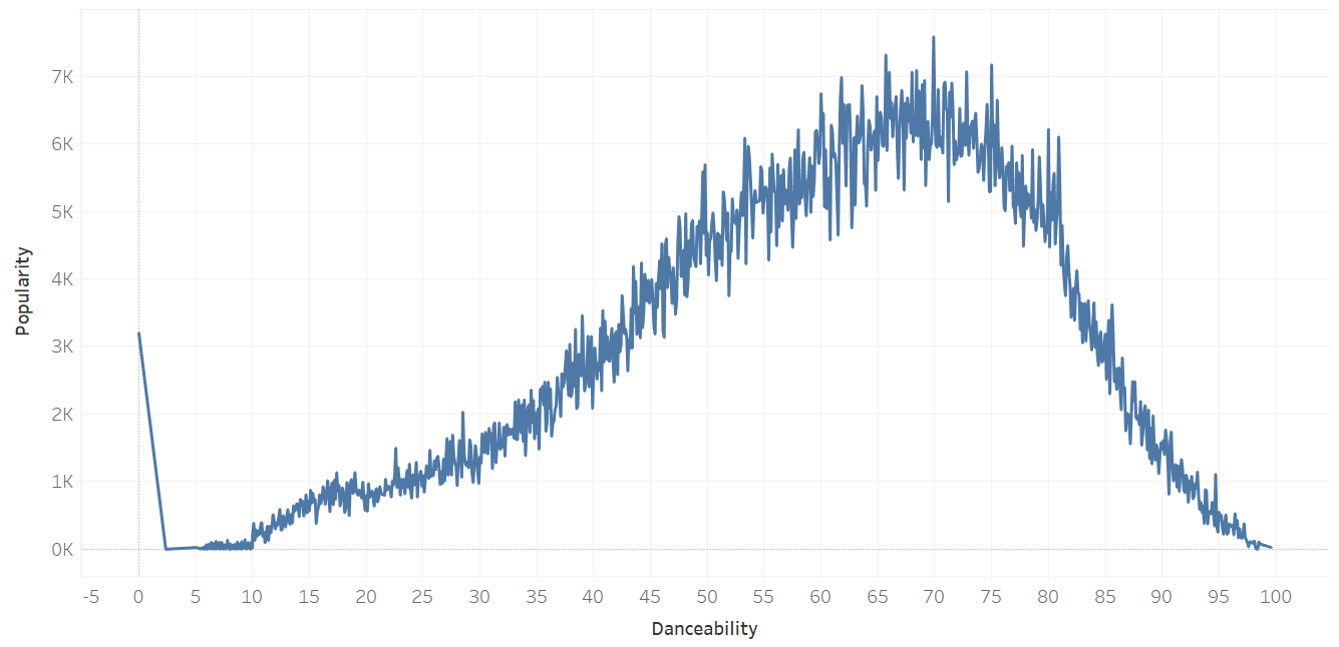
\includegraphics[width=1\linewidth]{./Slides/prz_dance} \end{center}

\end{frame}

\begin{frame}{How does mood affect the popularity of a song?}
\protect\hypertarget{how-does-mood-affect-the-popularity-of-a-song}{}

\begin{center}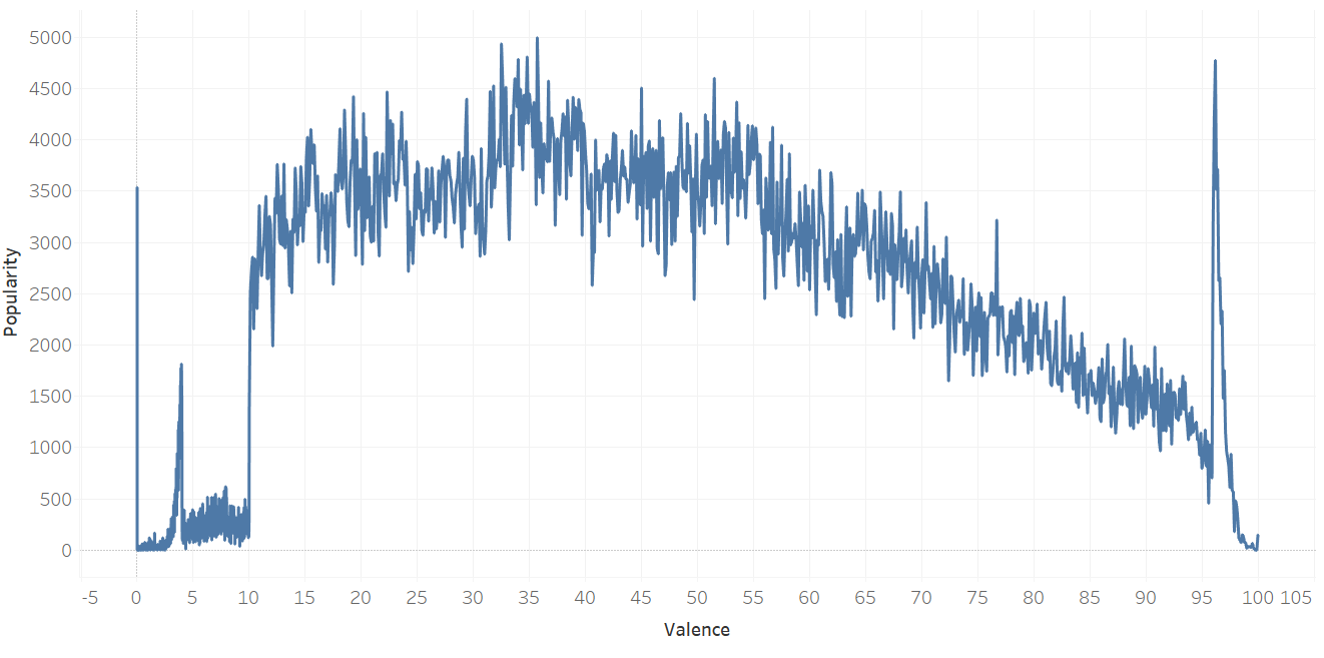
\includegraphics[width=1\linewidth]{./Slides/prz_mood} \end{center}

\end{frame}

\begin{frame}{Energy Vs. Popularity}
\protect\hypertarget{energy-vs.-popularity}{}

\begin{center}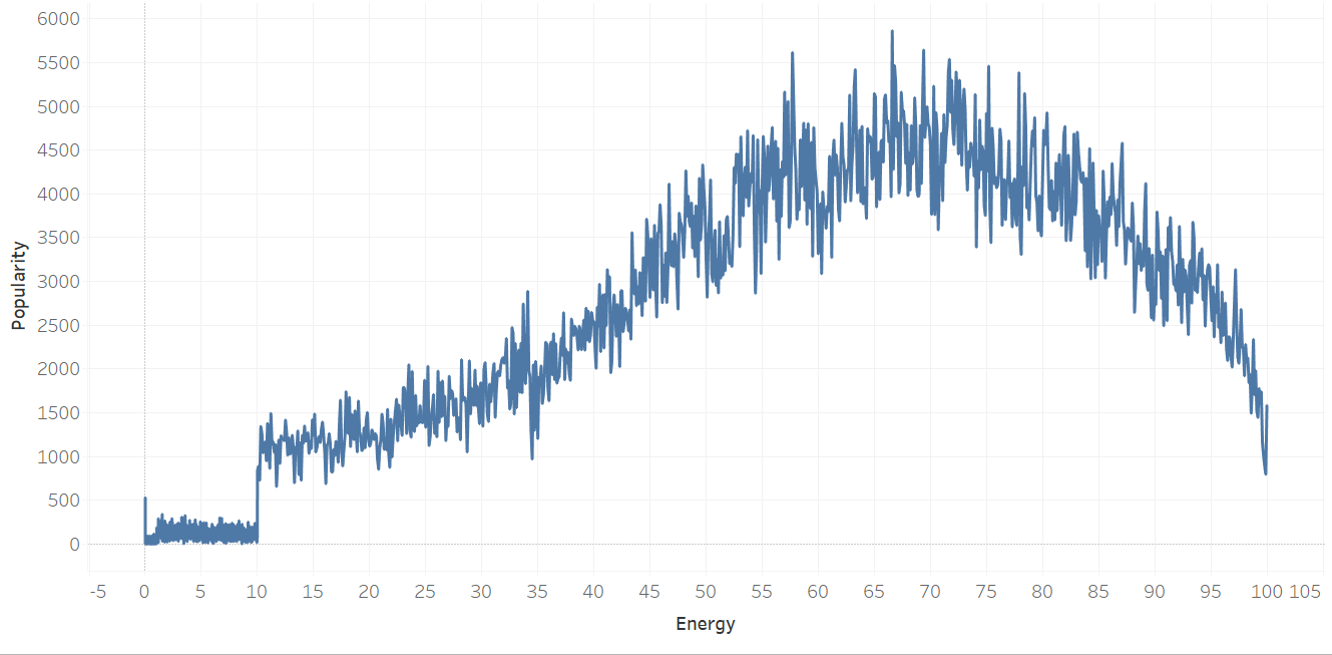
\includegraphics[width=1\linewidth]{./Slides/prz_energy} \end{center}

\end{frame}




\end{document}
